\chapter{Introduction}
MANDEYE DEV is 3D LiDAR (Light Detection and Ranging) data recorder introduced in ENRICH 2023 (https://enrich.european-robotics.eu/).
"ENRICH is the world's first and only robotics trial that gives you pure and unspoiled real world scenarios for testing." 
It can be mounted on any vehicle having 1kg payload or being hand held. 
MANDEYE DEV was integrated with small 4x4 autonomous mobile robot ClearPath Jackal. 
It received 3D mapping award after it delivers 3D map of the scenario in fully automatic way. 
It is robust, reliable, accurate, precise and 10x more affordable than competitive 3D mapping systems.
It can collect 3D data more than 4 hours in continuous mode.
The 3D map is processed off-line using open source software available in https://github.com/MapsHD/HDMapping/.
Data can be also converted to ROS rosbags (please send me email: januszbedkowski@gmail.com), so You can test it with plenty of LiDAR mapping open-source software.
It is designed for:

\begin{itemize}
	\item collecting 3D data for INDOOR and OUTDOOR scenes,
	\item providing ground-truth trajectory,
	\item enhance autonomous navigation and mapping of Your mobile robot,
	\item improve the robotic system deployment,
	\item professional applications,
	\item having fun from 3D mapping.
\end{itemize}
Following photos will show MANDEYE DEV and what it can do.
 %\begin{figure}[h]
% 	\centering
% 	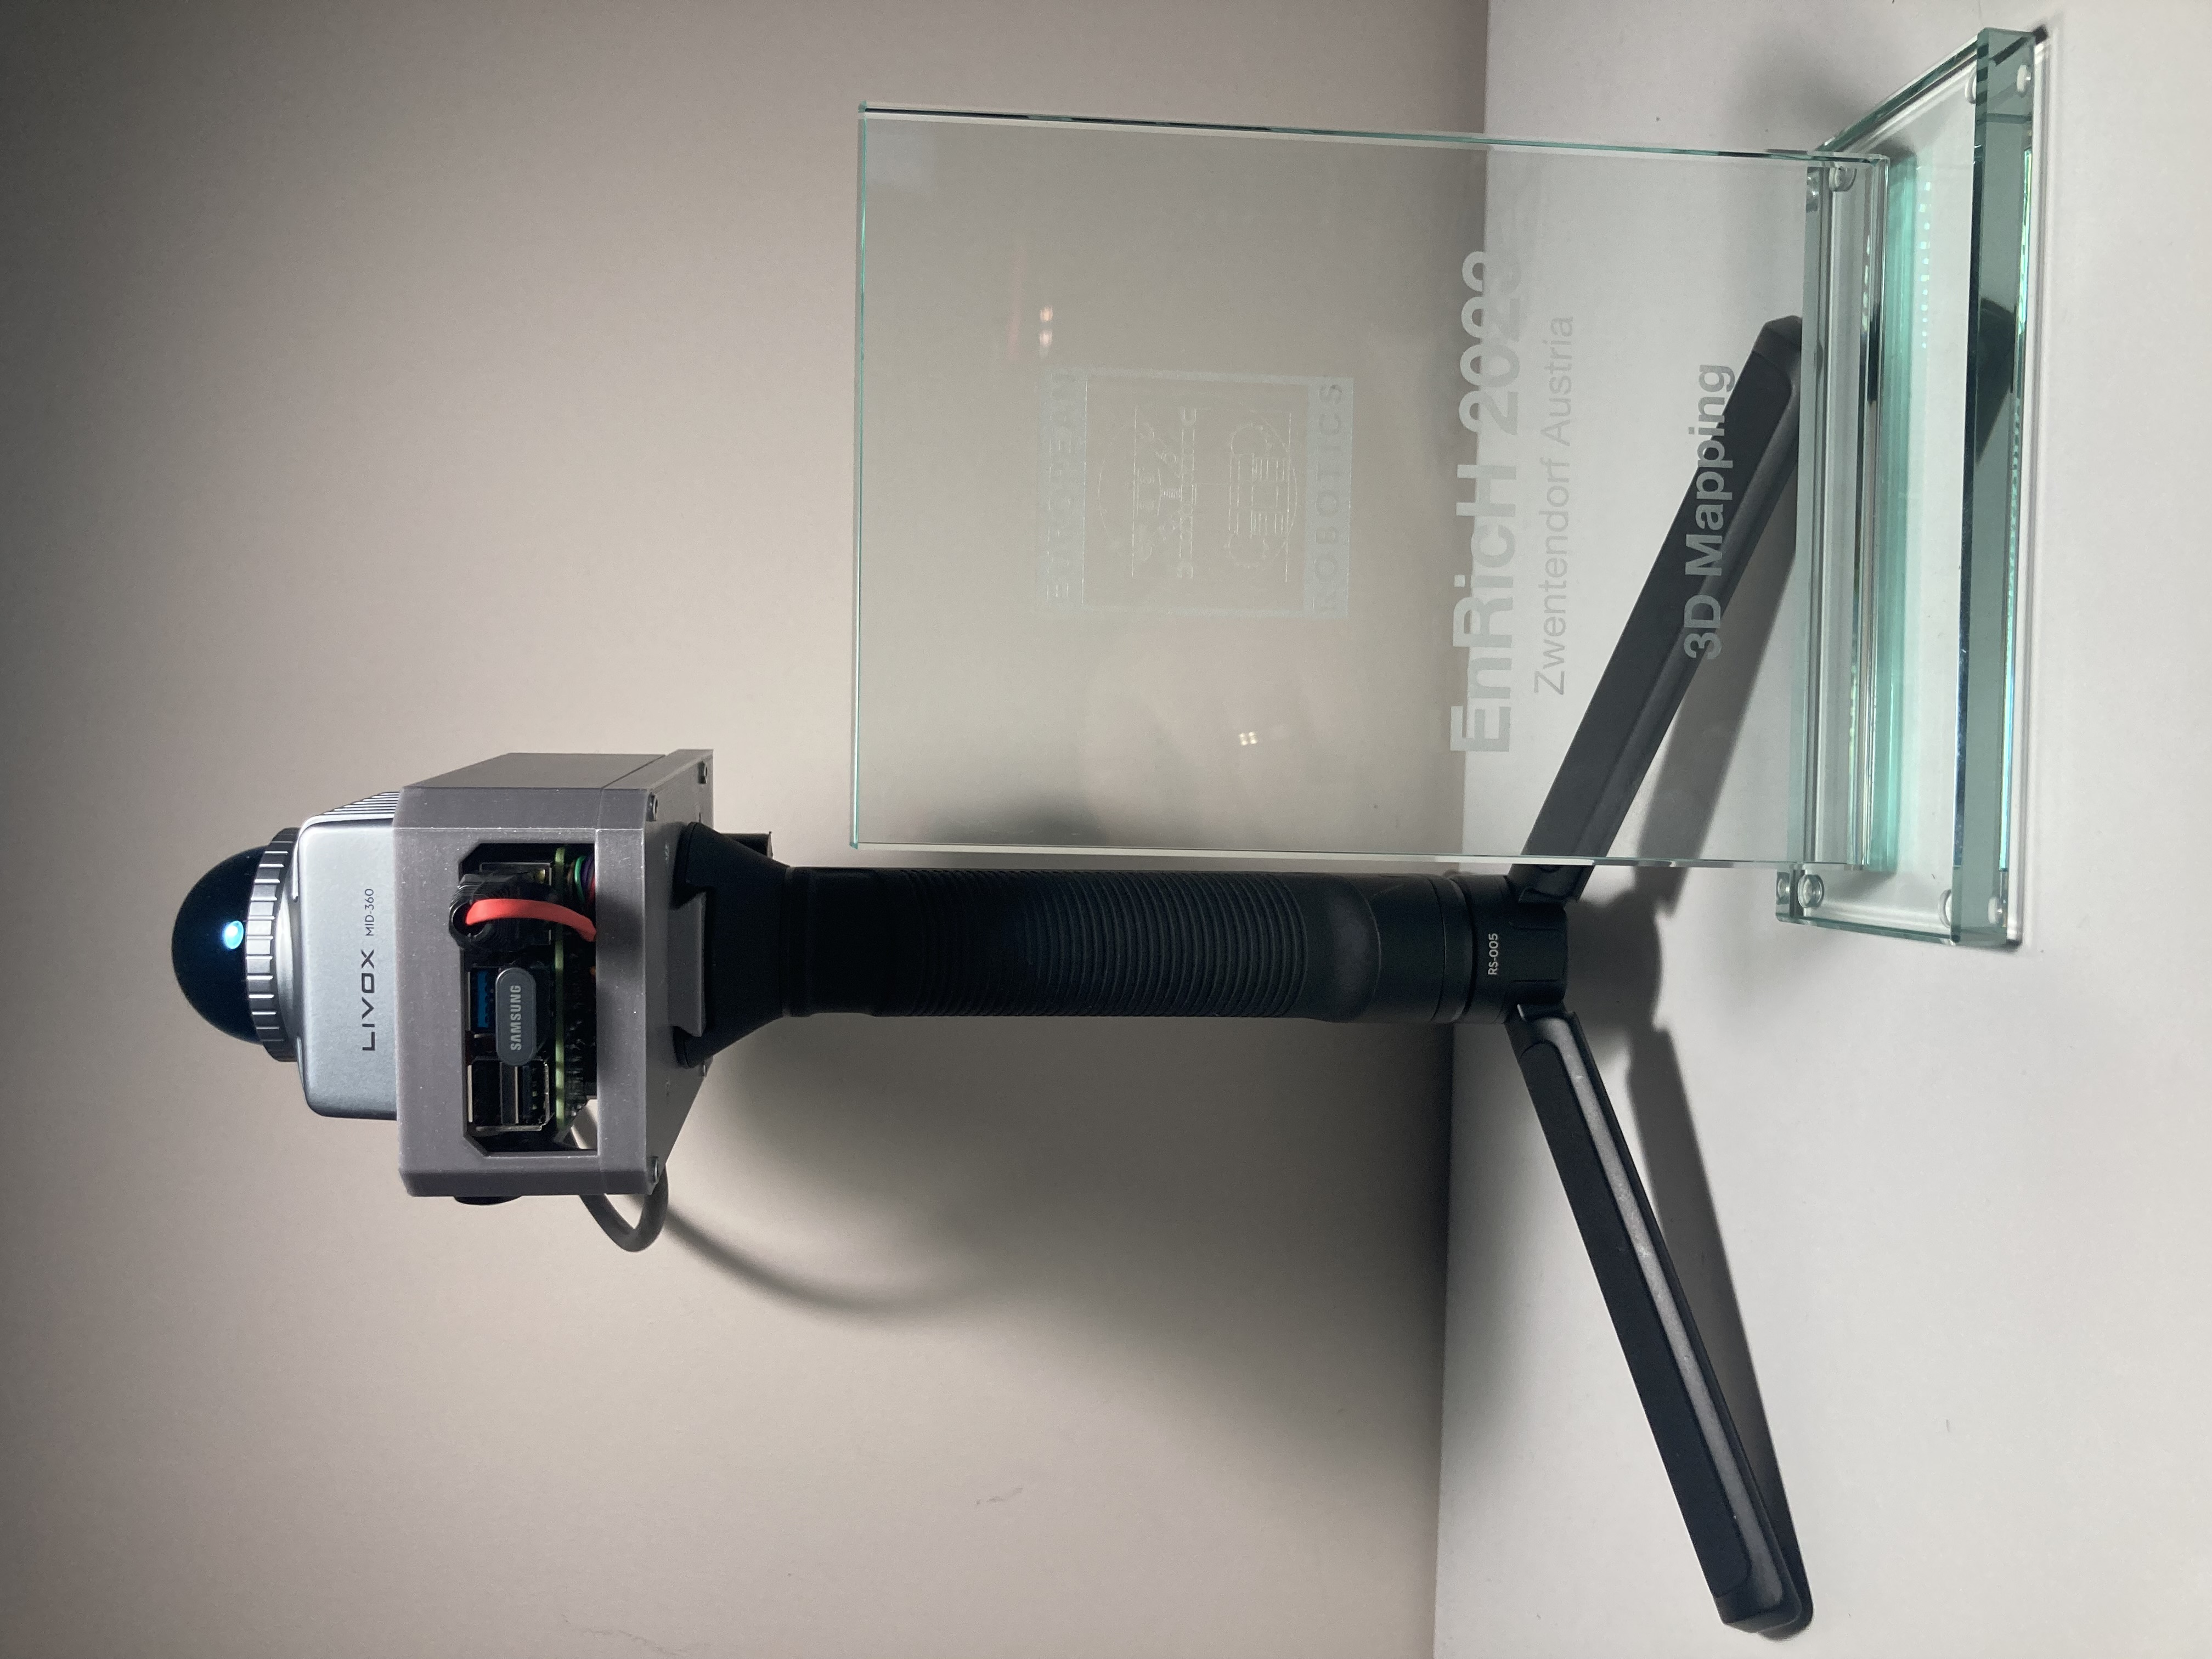
\includegraphics[width=0.5\textwidth, angle = -90]{IMG_9490.jpg}
% 	\caption{MANDEYE DEV - 3D LiDAR (Light Detection and Ranging) data recorder awarded in ENRICH 2023 (https://enrich.european-robotics.eu/).}
% 	\label{fig:mesh1}
% \end{figure}


 \begin{figure}
 	\centering
 	\begin{subfigure}[b]{0.4\textwidth}
 		\centering
 		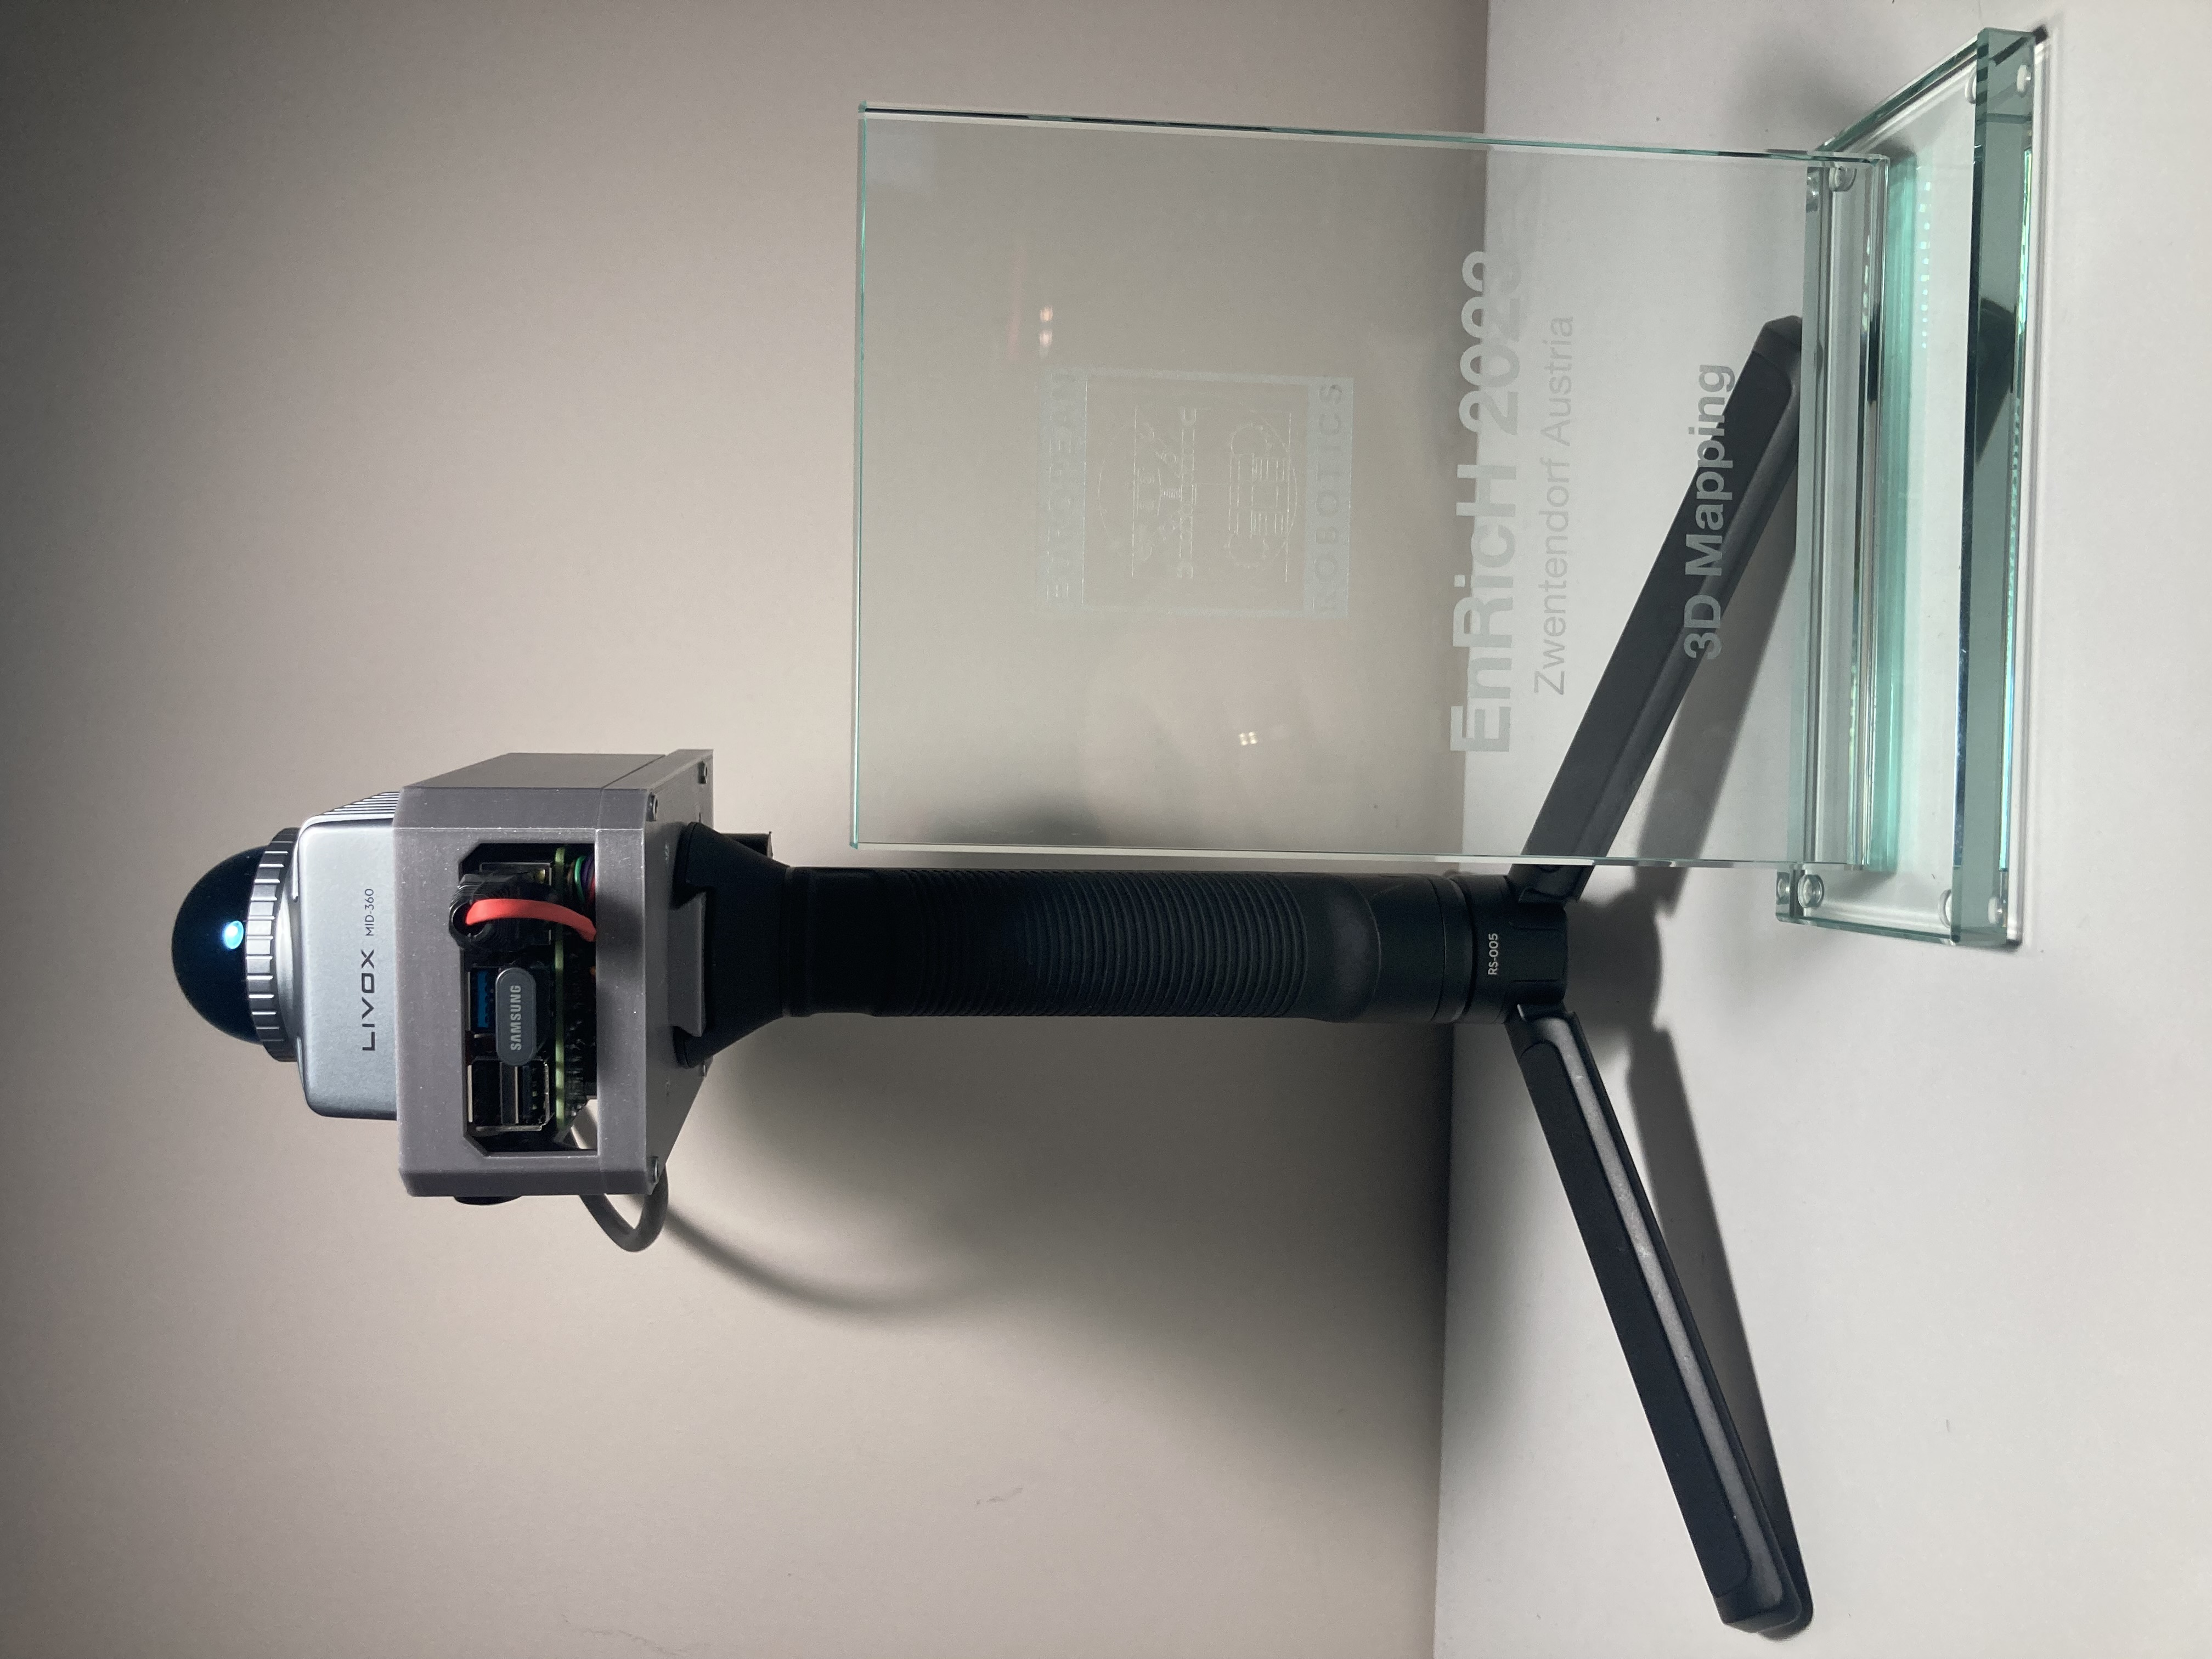
\includegraphics[width=\textwidth, angle = -90]{IMG_9490.jpg}
 		\caption{MANDEYE DEV with 3D mapping award.}
 		\label{fig:a}
 	\end{subfigure}
 	\hfill
 	\begin{subfigure}[b]{0.4\textwidth}
 		\centering
 		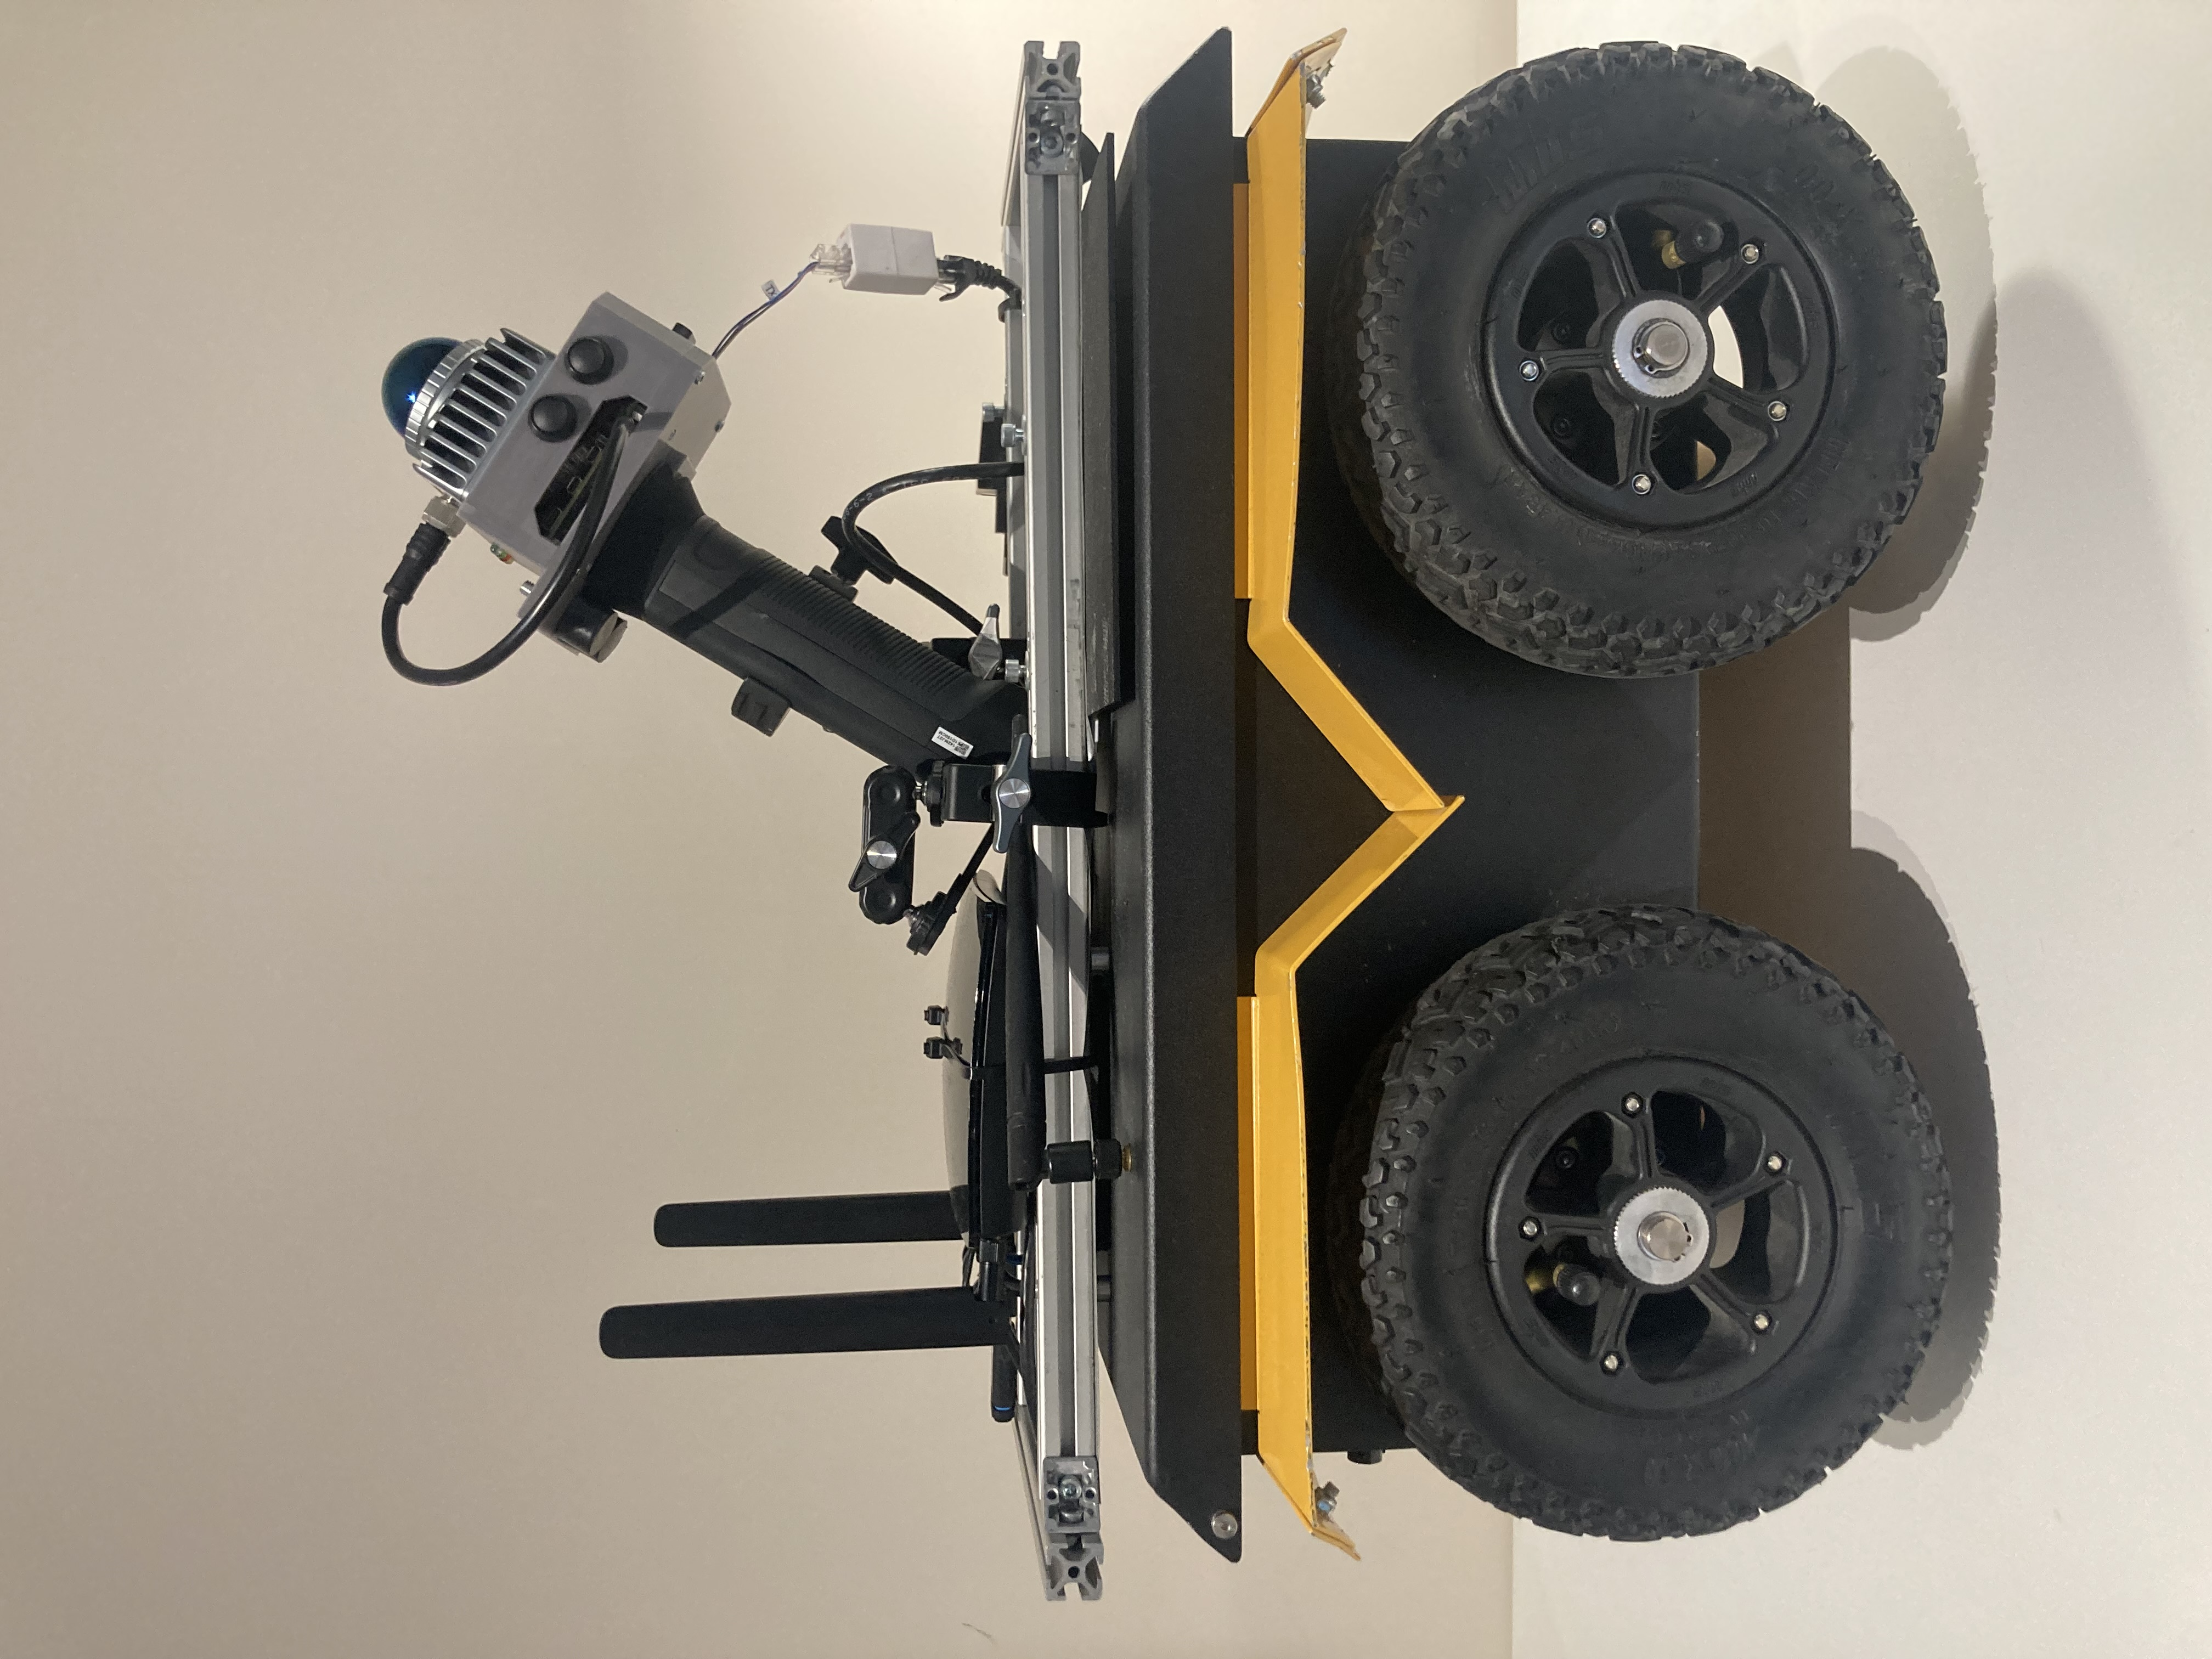
\includegraphics[width=\textwidth, angle = -90]{IMG_9492.jpg}
 		\caption{MANDEYE DEV integrated with 4x4 Jackal robot.}
 		\label{fig:b}
 	\end{subfigure}
 	\hfill
 	\begin{subfigure}[b]{0.7\textwidth}
 		\centering
 		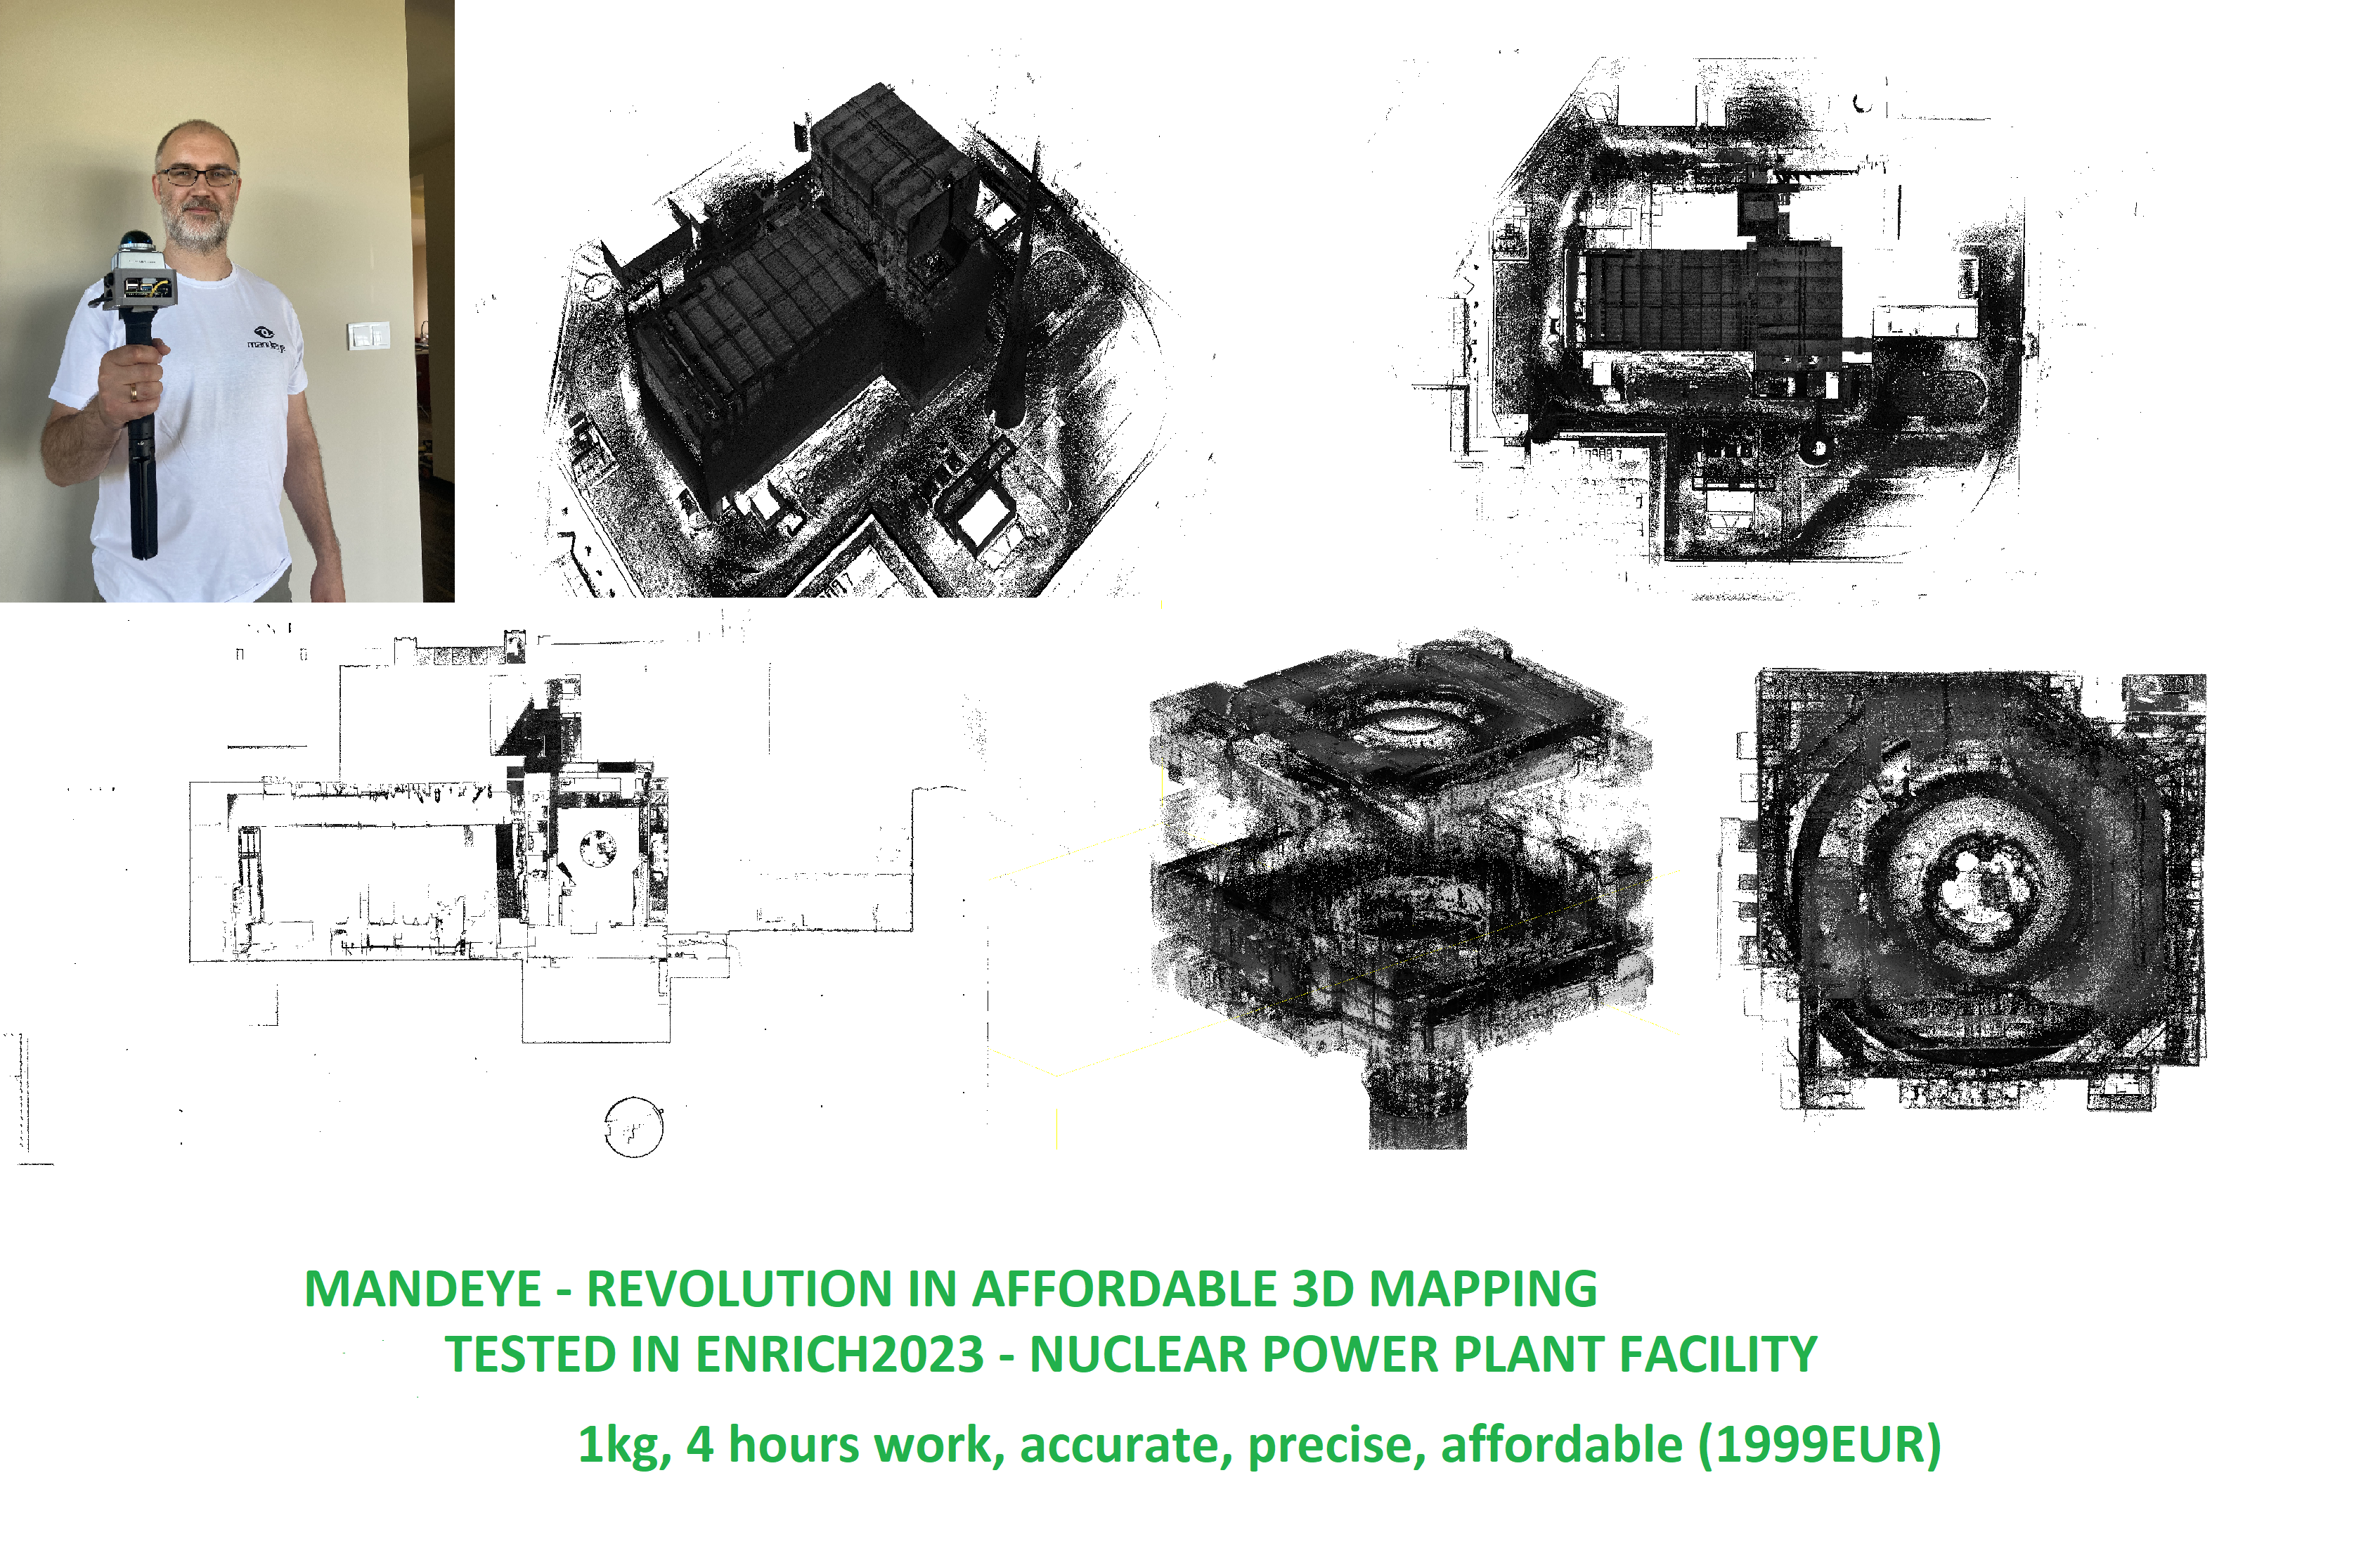
\includegraphics[width=\textwidth]{mandeye_npp.png}
 		\caption{3D map of entire Nuclear Plant acquired with hand-held MANDEYE DEV.}
 		\label{fig:c}
 	\end{subfigure}
 	\hfill
 	\begin{subfigure}[b]{0.7\textwidth}
 		\centering
 		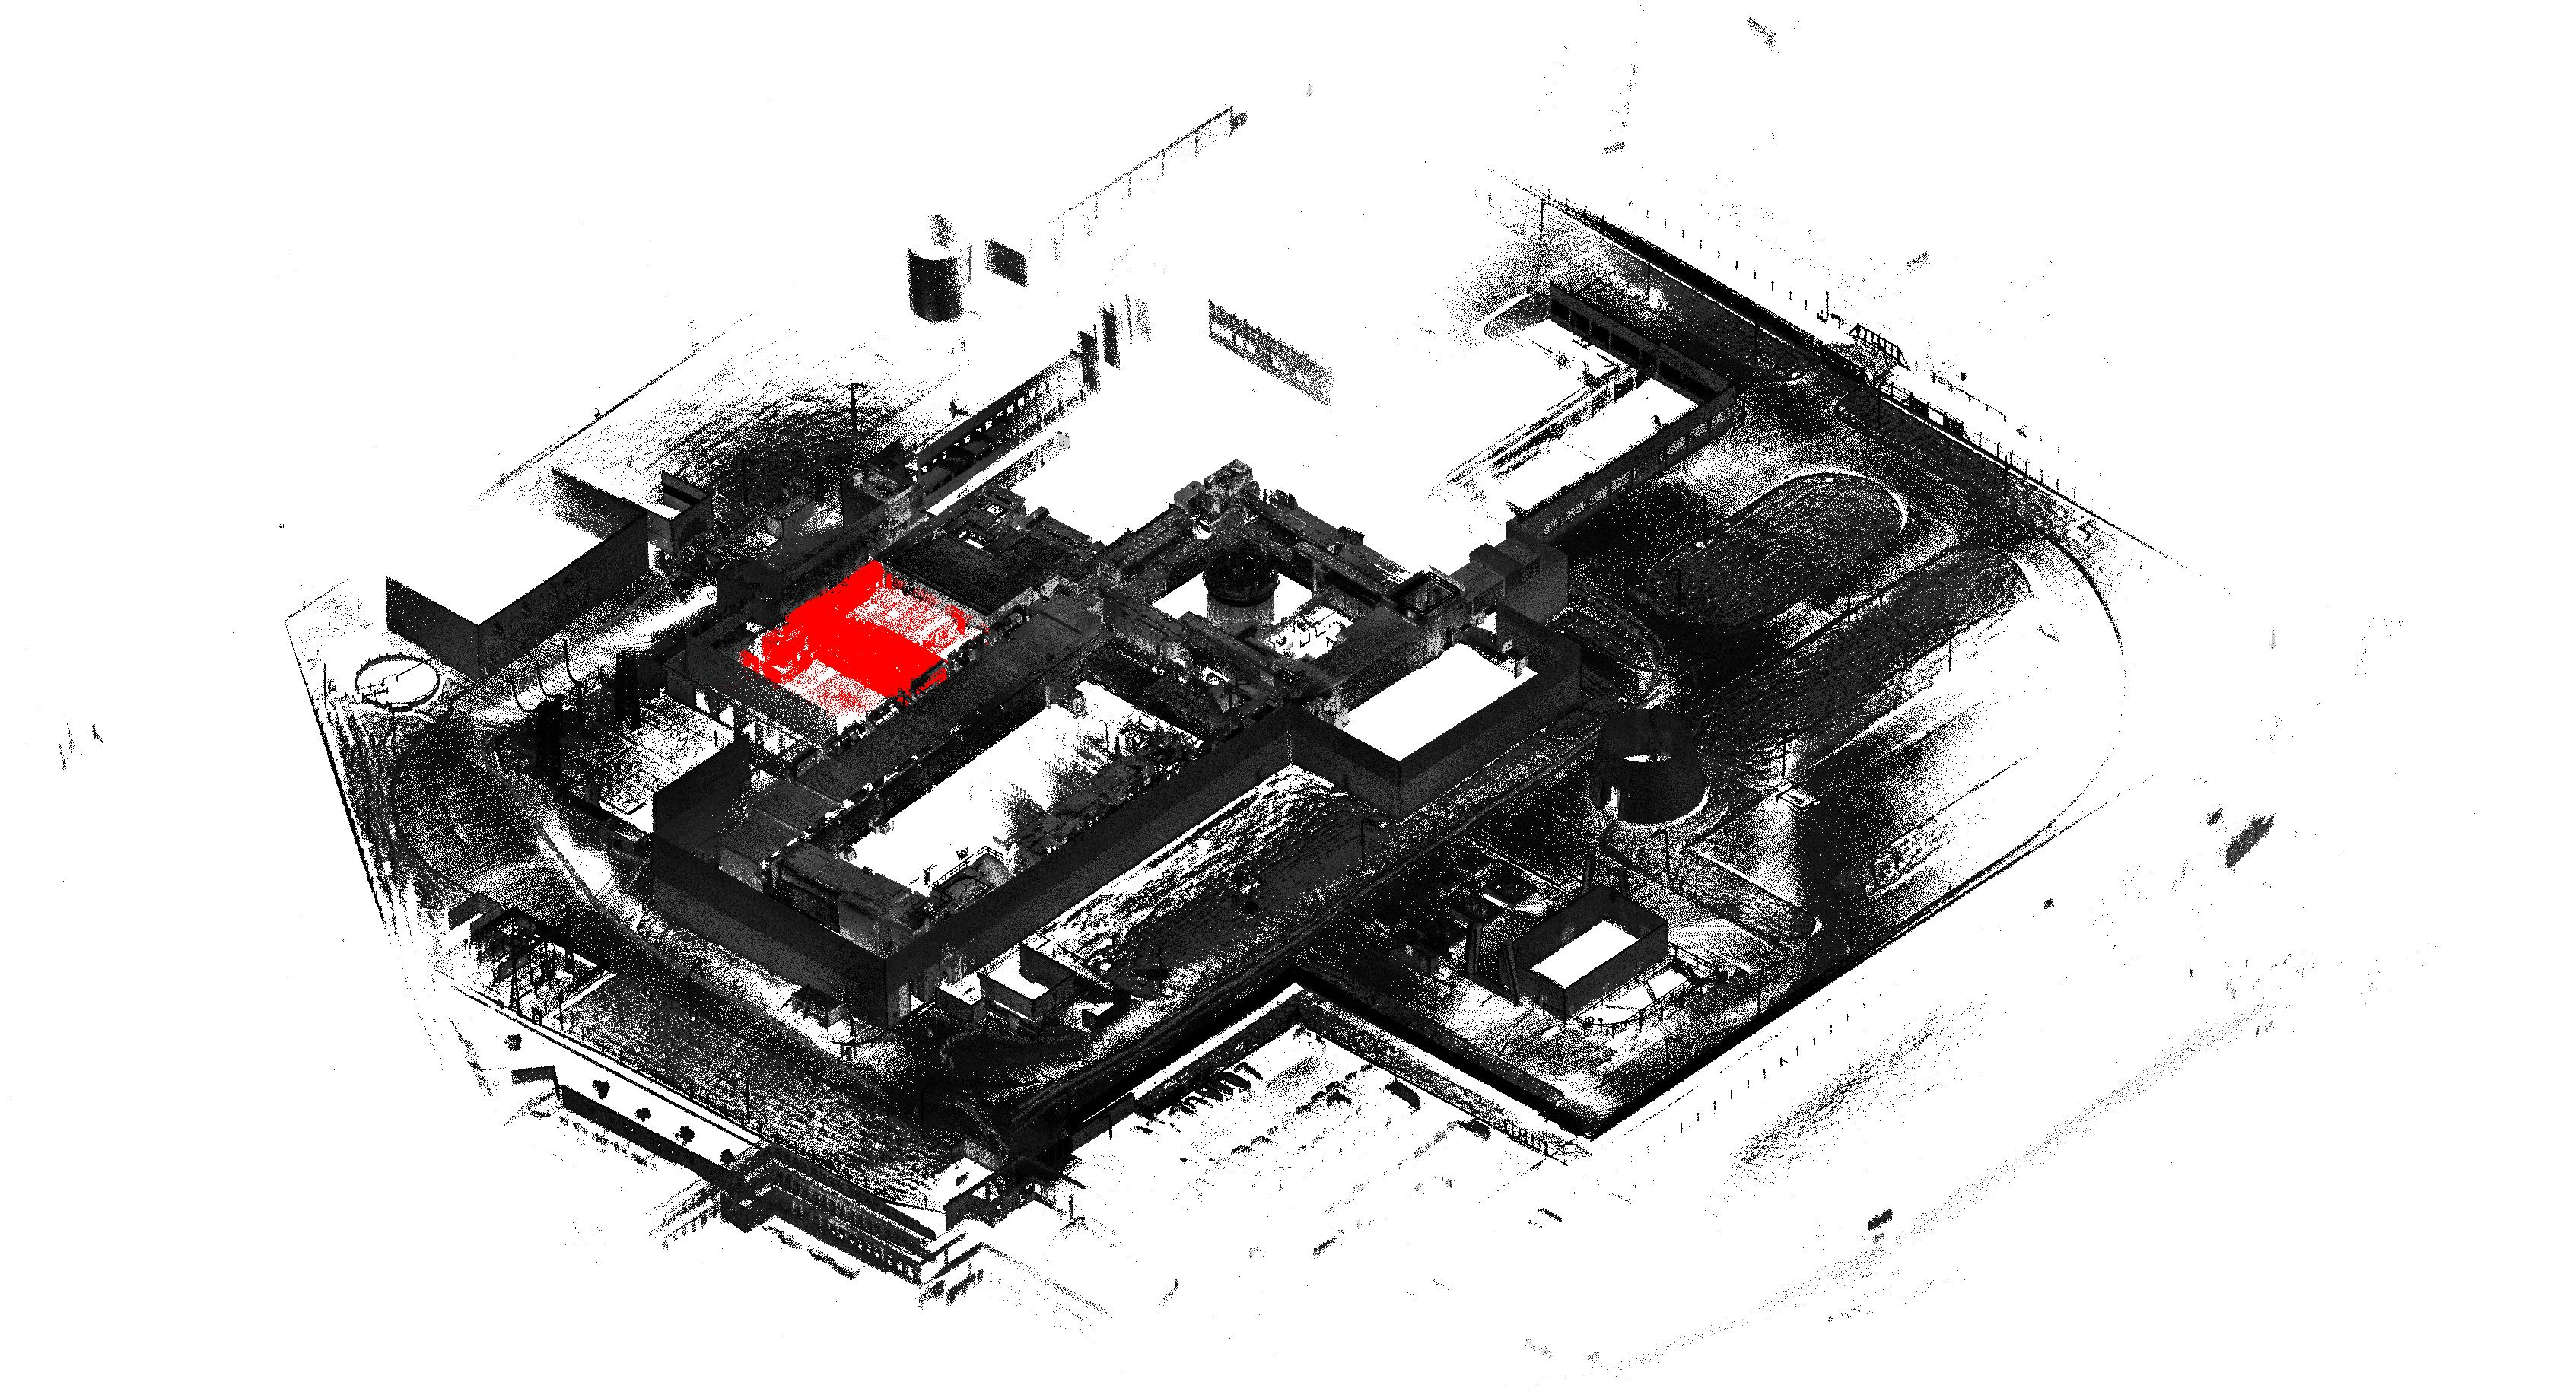
\includegraphics[width=\textwidth]{npp_all_madeye_jackal.jpg}
 		\caption{Red color: 3D map delivered by autonomous 4x4 Jackal equipped with MANDEYE DEV. Gray scale: 3D map of ground floor of Nuclear Plant acquired with hand-held MANDEYE DEV.}
 		\label{fig:d}
 	\end{subfigure}
  	\caption{MANDEYE DEV for professional use in action during ENRICH 2023 https://enrich.european-robotics.eu/.}
 	\label{fig:abcd}
 \end{figure}

\begin{figure}
	\centering
	\begin{subfigure}[b]{0.4\textwidth}
		\centering
		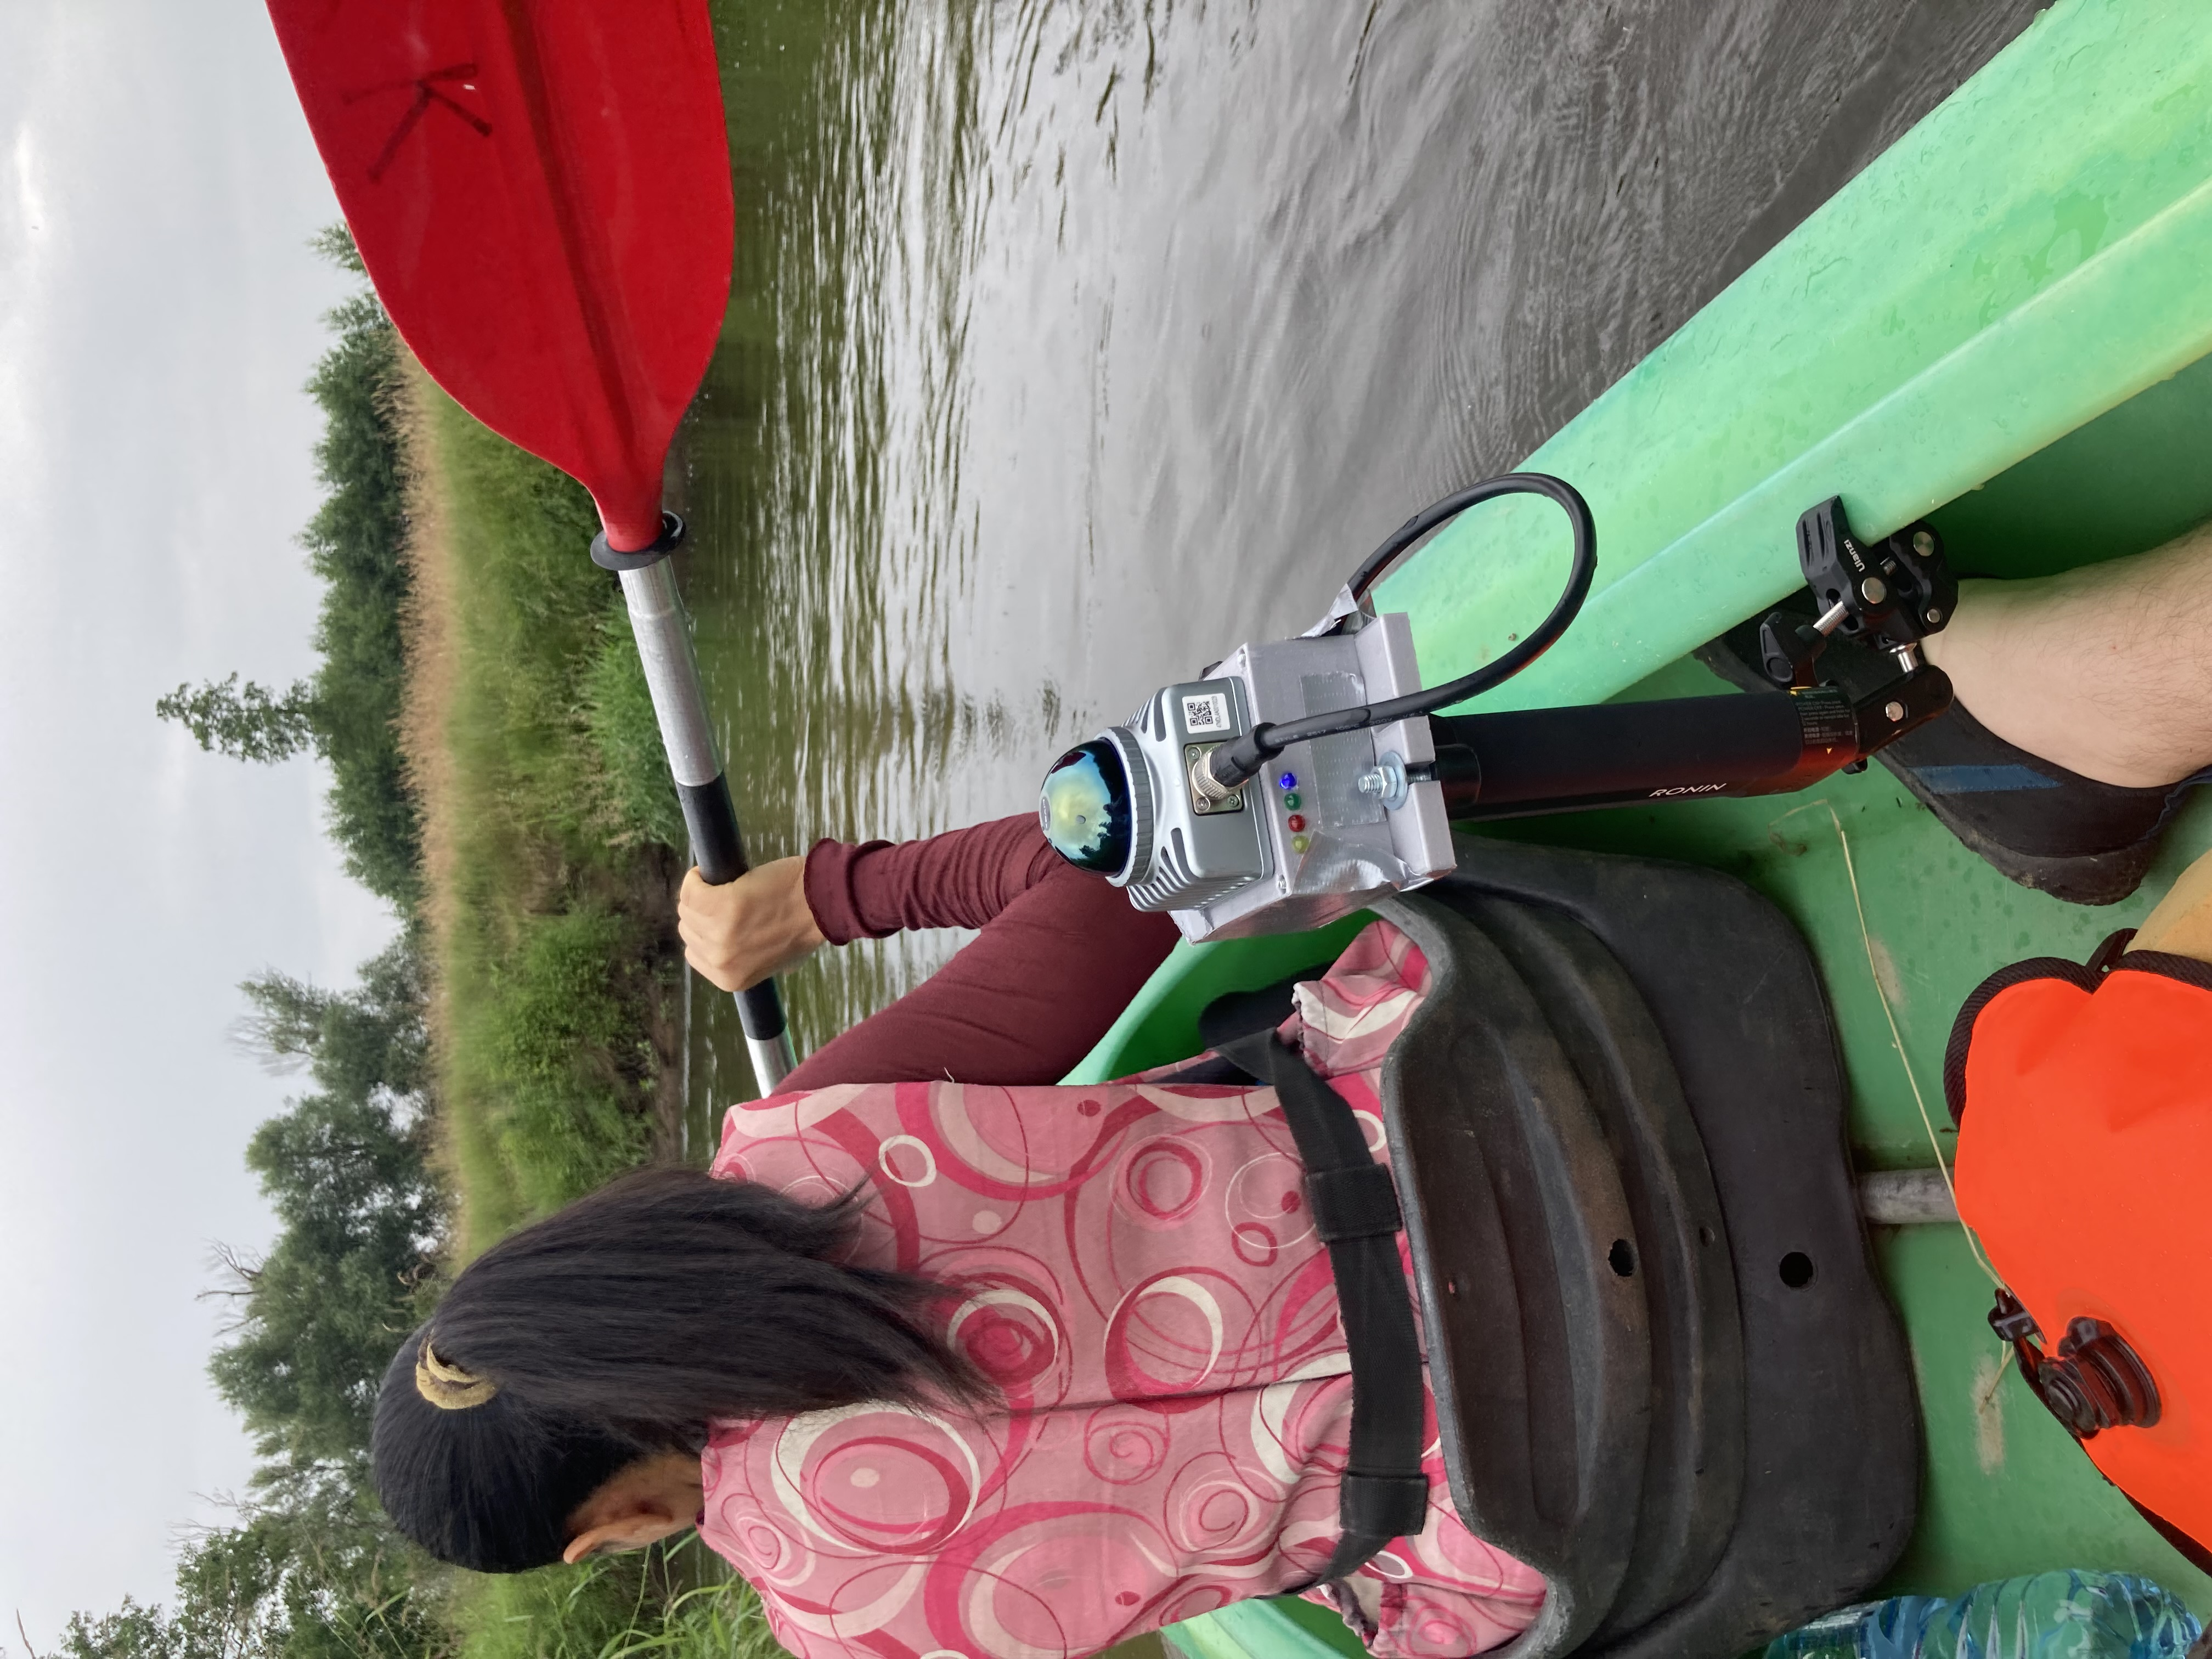
\includegraphics[width=\textwidth, angle = -90]{IMG_9458.jpg}
		\caption{MANDEYE DEV mounted onto water vessel.}
		\label{fig:a2}
	\end{subfigure}
	\hfill
	\begin{subfigure}[b]{0.7\textwidth}
		\centering
		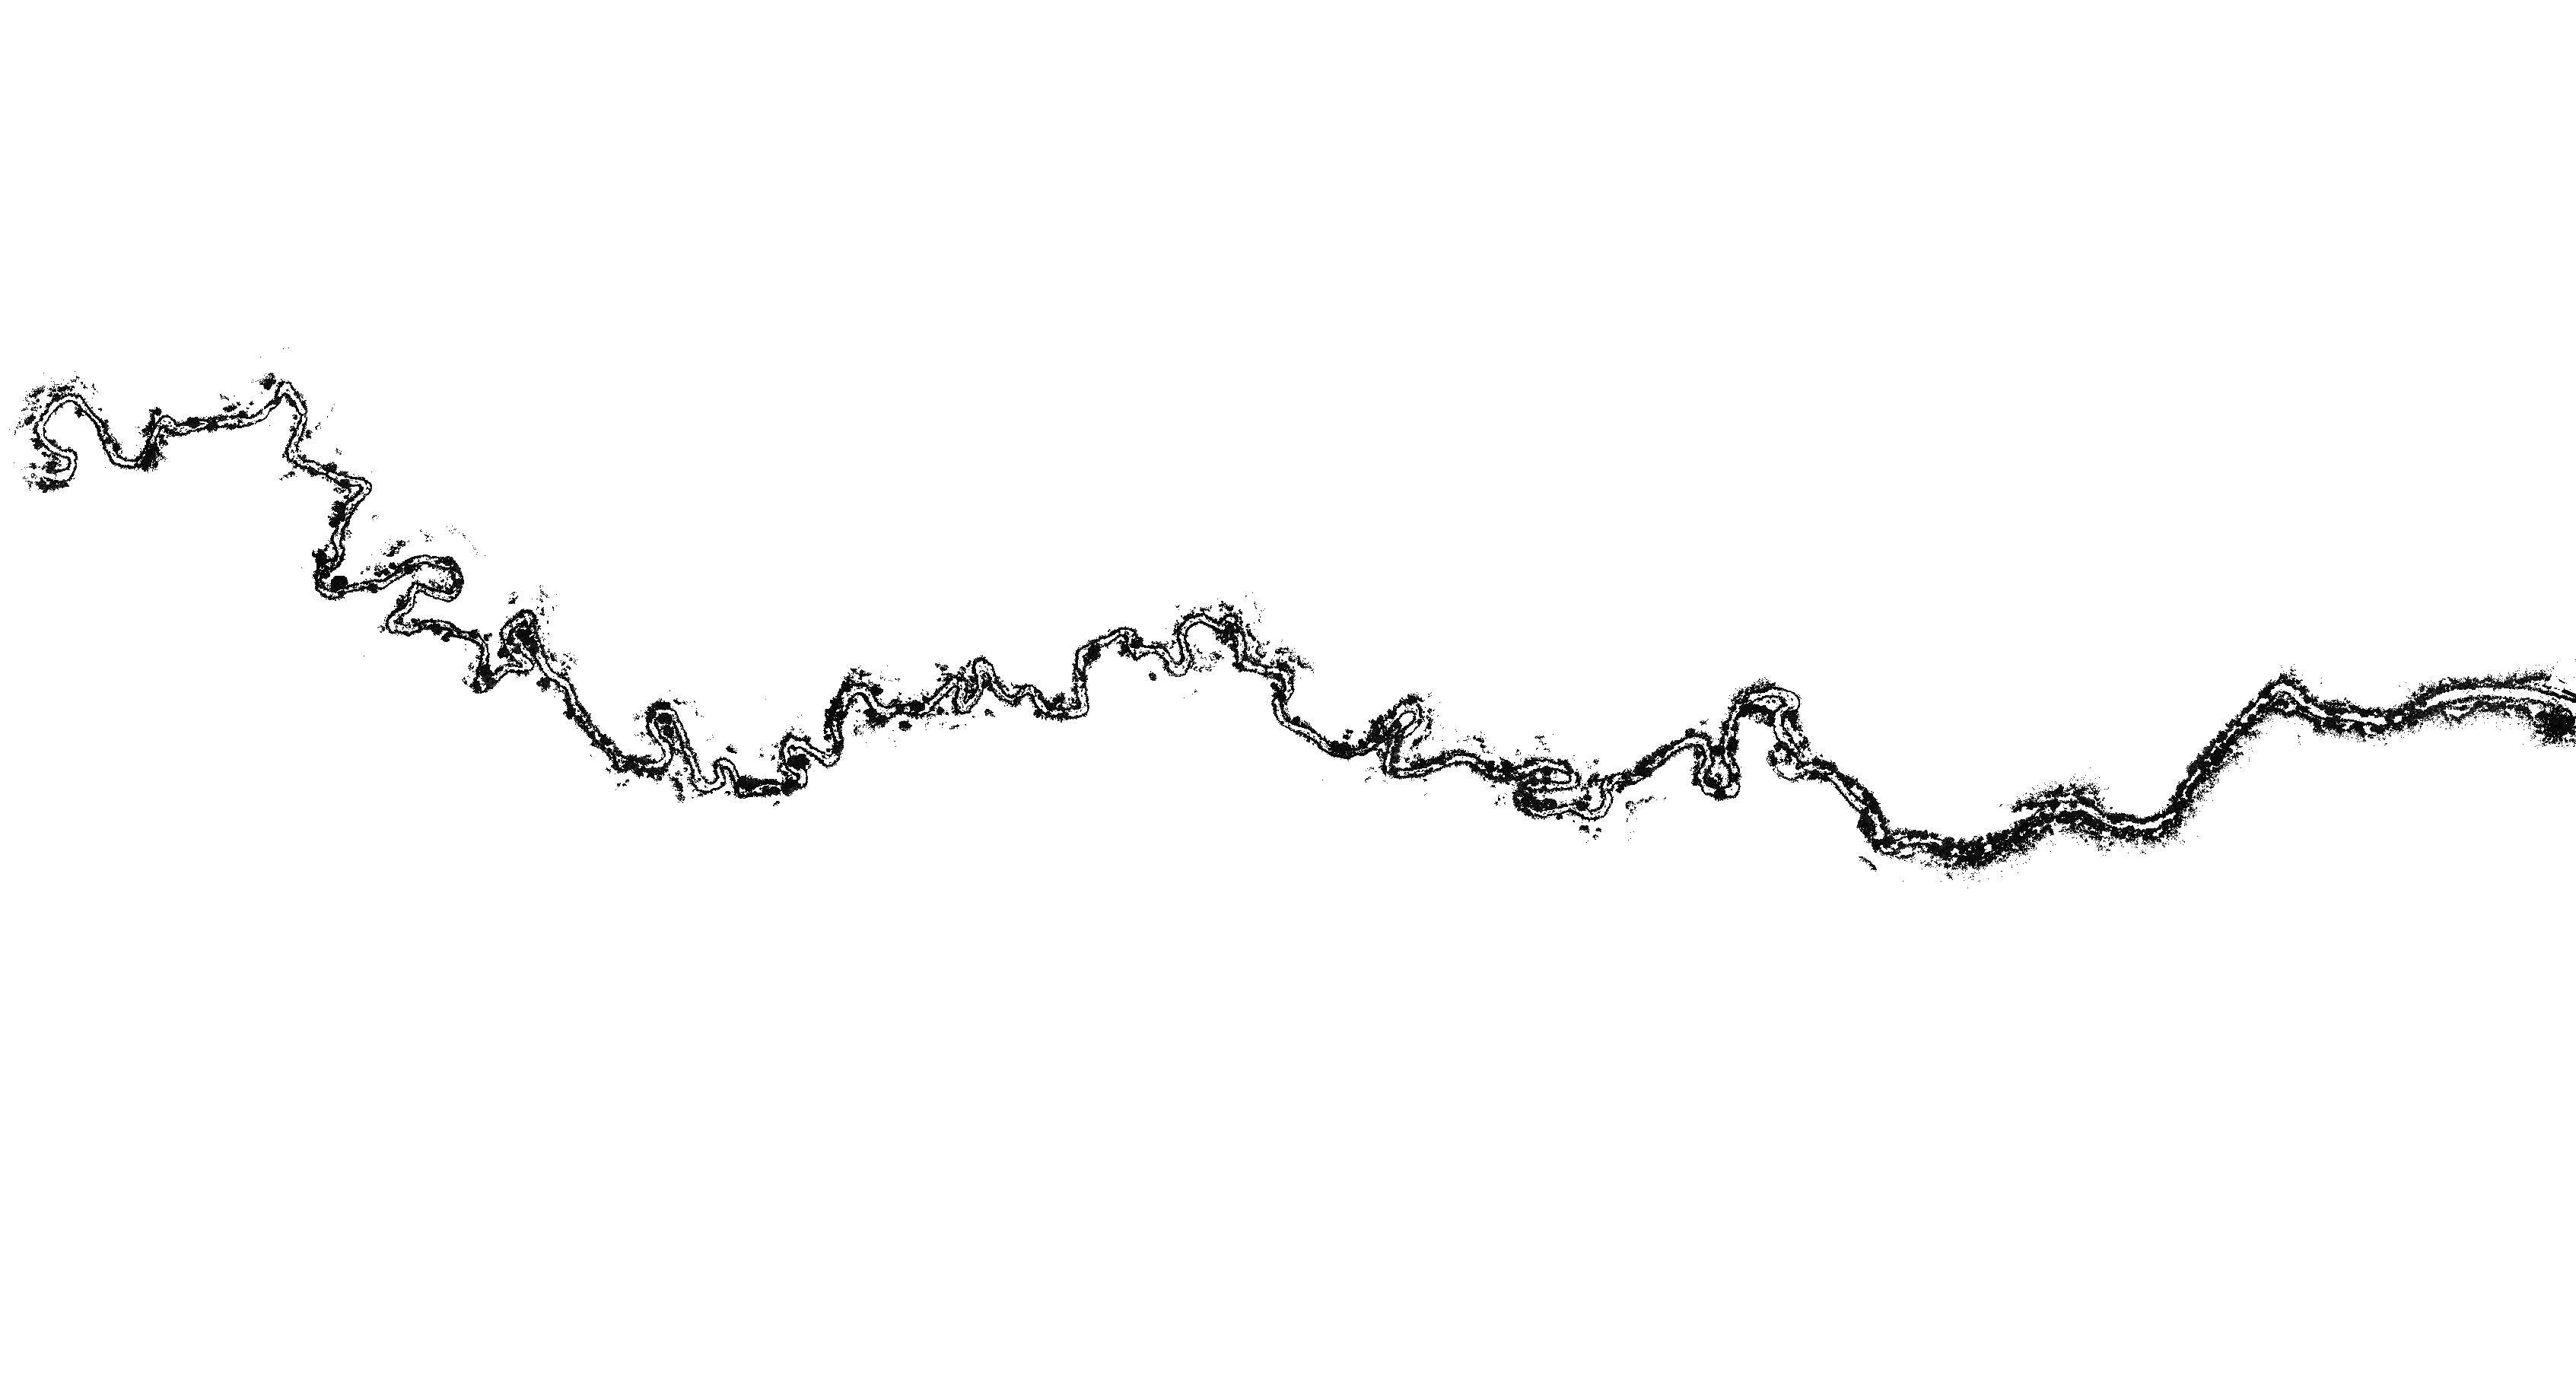
\includegraphics[width=\textwidth]{river.jpg}
		\caption{3km river trip.}
		\label{fig:b2}
	\end{subfigure}
	\hfill
	\begin{subfigure}[b]{0.7\textwidth}
		\centering
		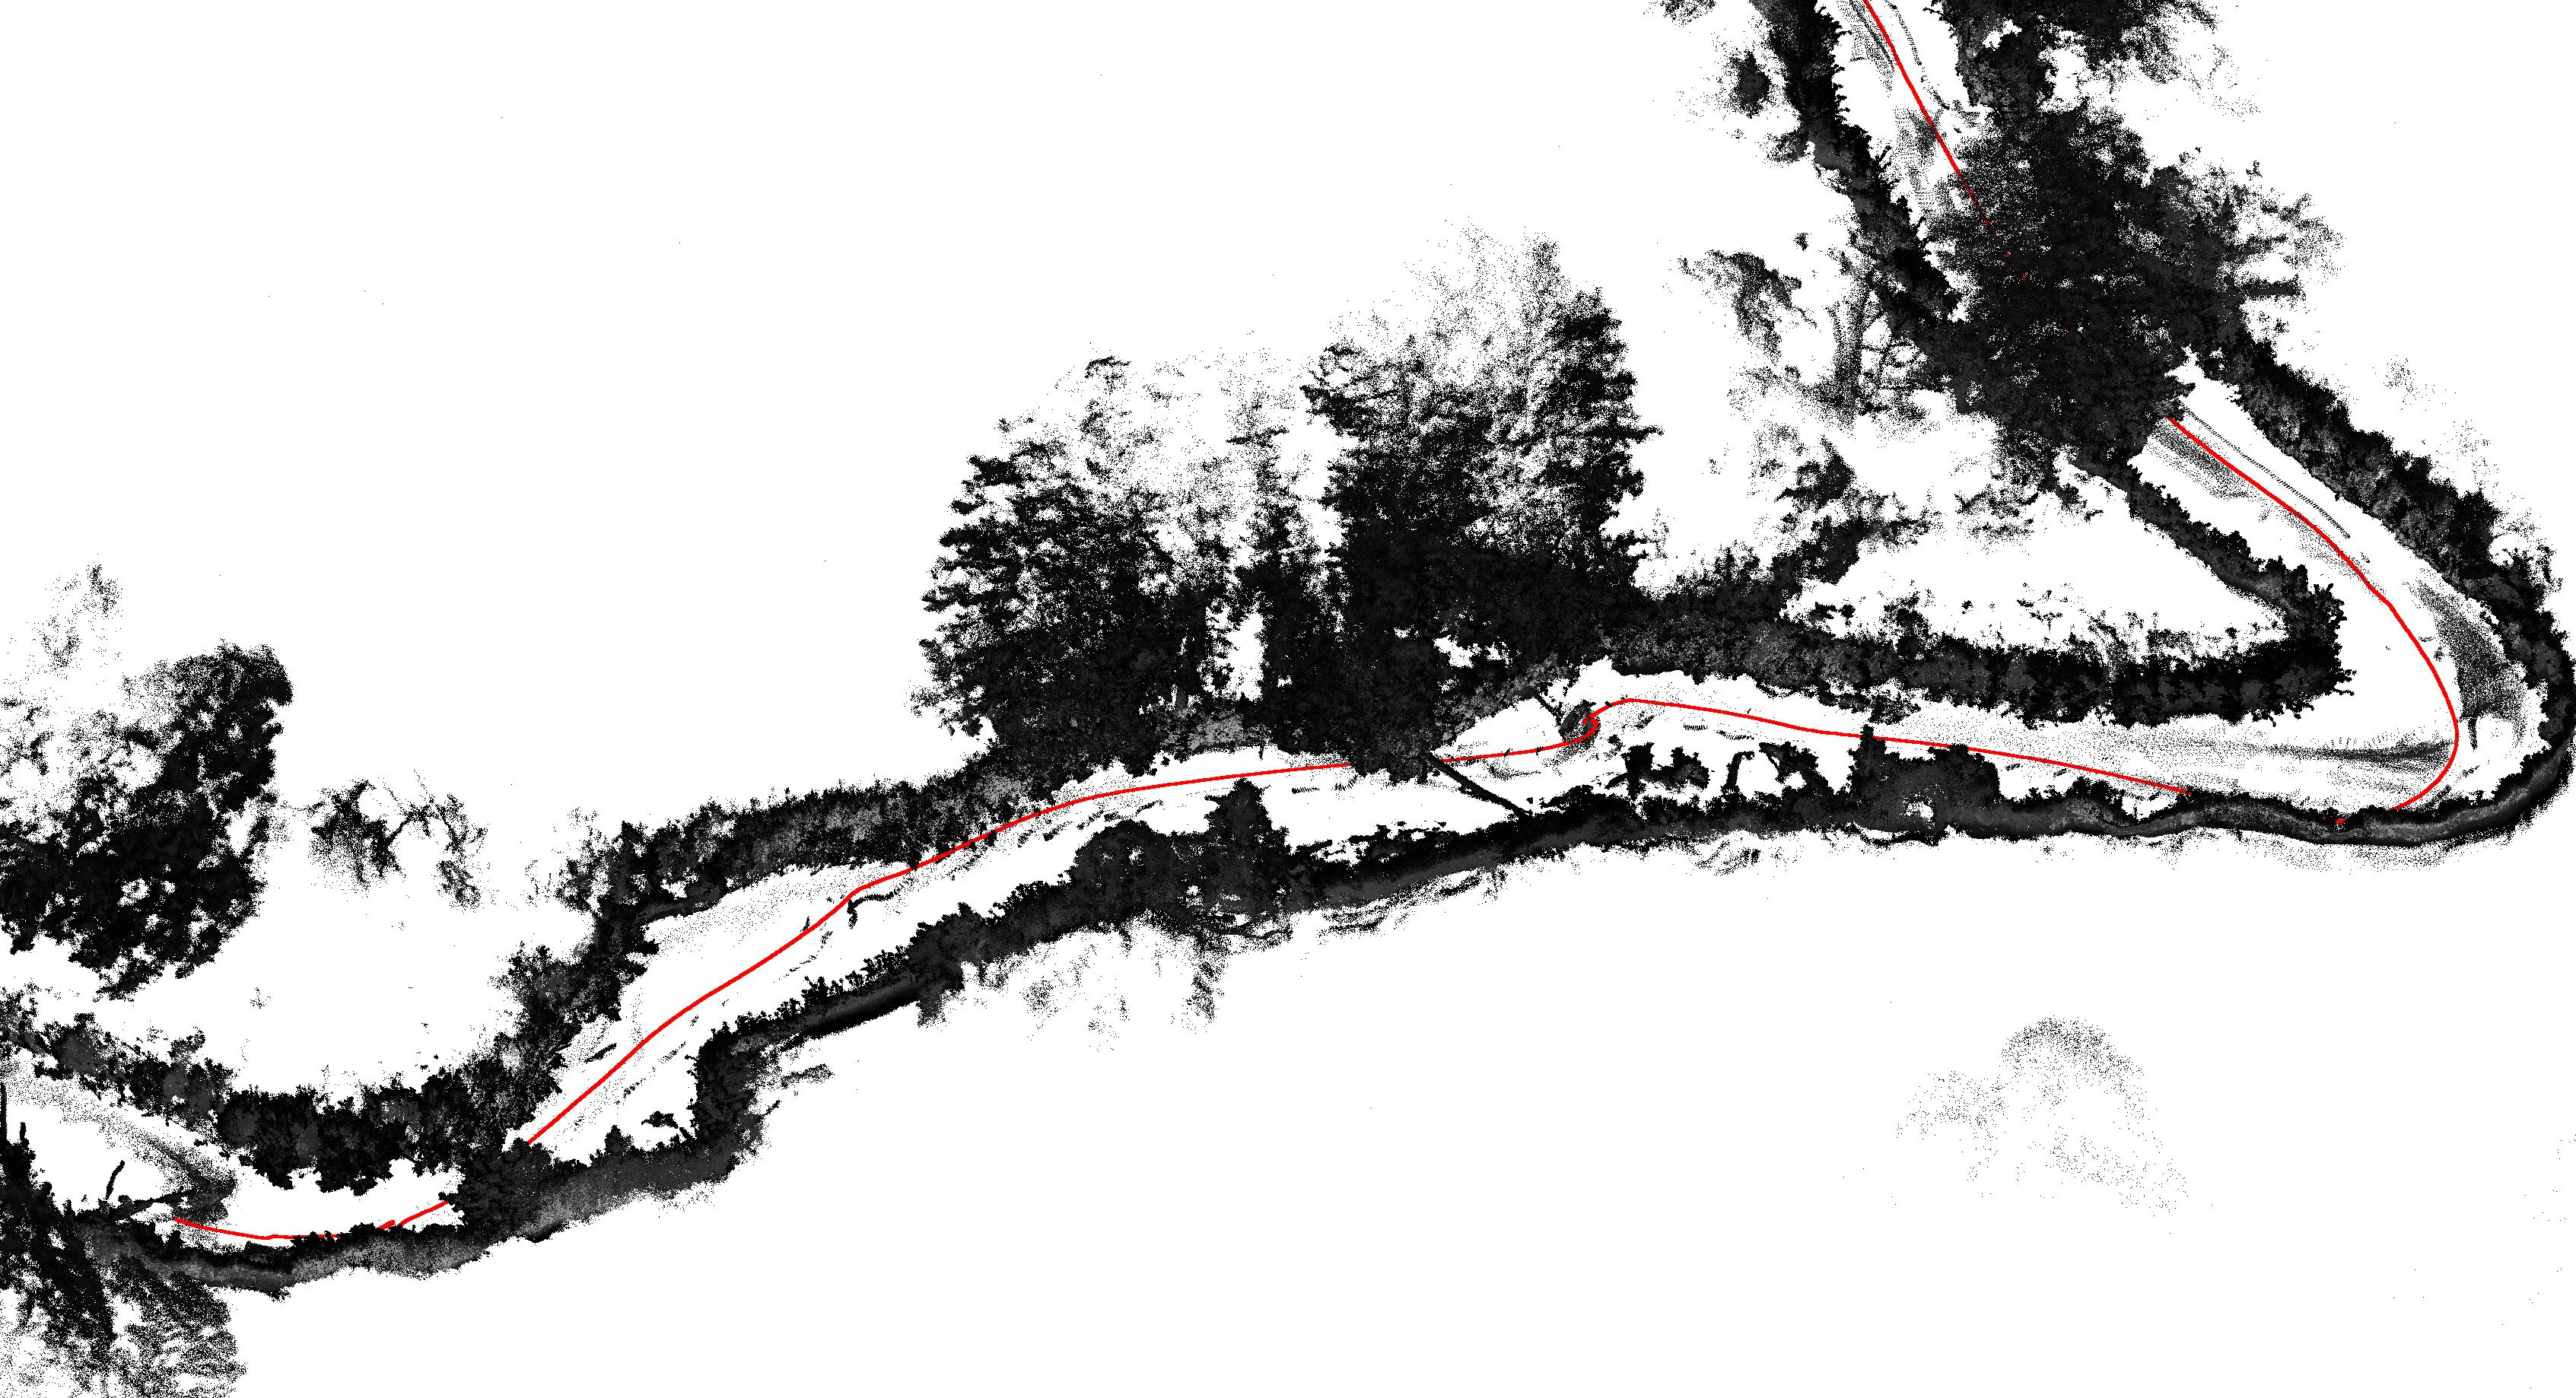
\includegraphics[width=\textwidth]{river2.jpg}
		\caption{Red line: ground truth trajectory of water vessels. Gray scale: 3D map.}
		\label{fig:c2}
	\end{subfigure}
	\caption{MANDEYE DEV for having fun with 3D mapping.}
	\label{fig:a2b2c2}
\end{figure}

